\documentclass[14pt,titlepage, a4paper]{extarticle}
\usepackage{tikz}
\usetikzlibrary{shapes.geometric, arrows, positioning}

% tikz styling
\tikzstyle{block} = [rectangle, 
			draw, 
			rounded corners, 
			text centered, 
			minimum height = 2em]
\tikzstyle{rect} = [rectangle, 
			draw, 
			text centered, 
			minimum height = 2em]
\tikzstyle{nrect} = [rectangle, 
			text centered, 
			minimum height = 2em]
\tikzstyle{line} = [draw, -latex']

\title{Networks Lab Report\\Assignment 2}
\author{Md Sahil\\BCSE III\\Roll-001710501029}
\date{}

\begin{document}

{\maketitle}

\section{Objectives}
Implement three data link layer protocols, 
Stop and Wait, 
Go Back N Sliding Window 
and Selective Repeat Sliding Window for flow control.

\section{Design and Implementation}

\subsection{Program structure}
The implementation is done using sockets.
The clients and server communicate with each other using sockets.
Listening on the channel is done through a separate 
thread (for both client and server).
There can be multiple client instances. All the clients are connected to the
central server.


\subsubsection{The Server class}
The server class instance acts as a medium to connect two clients. 
Whenever the server is starts listening and accepting client socket
connections. Each time a client connection is made, its control is
passed on to the client handler thread. The client handler thread then 
listens for incoming frames from the assigned client socket.
The server also maintains a list of mappings of clients with port 
numbers and client addresses. When ever a client tries to connect to a server. 
The server maps the port number with the client address.
When a client tries to sent messages to another client, the server checks the
destination address of the message, finds the port mapped to the address
and forwards the message to the destination client.
\par\null\par
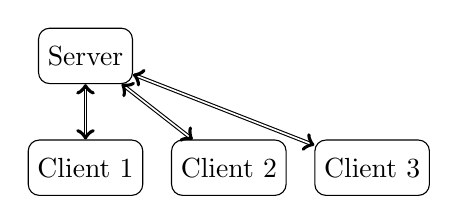
\begin{tikzpicture}[node distance = 1em, auto]
	\node [block] (server) {Server};
	\node [block, below=2em of server] (client1) {Client 1};
	\node [block, right=of client1] (client2) {Client 2};
	\node [block, right=of client2] (client3) {Client 3};
	\draw [double,<->] (server) -- (client1);
	\draw [double,<->] (server) -- (client2);
	\draw [double,<->] (server) -- (client3);
\end{tikzpicture}

\subsubsection{The Client class}
The client class provides all the basic infrastructure
for communication with the server. Listening is done on a separate
thread for each client. Whenever a client tries to connect to a server,
it sends a request to connect frame which contains the address of the client.
In the server side, the server registers the port number and the address in its
address list and sends back an request accept frame.
\\
The Client class has six specialization subclasses.
Each pair of subclass (a sender client and a receiver client) implements
one of the three data link layer protocols.
\begin{description}
	\item [Stop and Wait] in  SAWSenderClient and SAWReceiverClient
	\item [Go back N] in GNSenderClient and GNReceiverClient
	\item [Selective Repeat] in SRSenderClient and SRReceiverClient
\end{description}

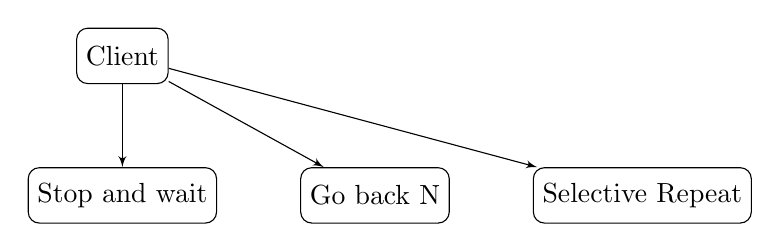
\begin{tikzpicture}[node distance = 3em, auto]
	\node [block] (clientClass) {Client};
	\node [block, below=of clientClass] (SAW) {Stop and wait};
	\path [line] (clientClass) -- (SAW);
	\node [block, right=of SAW] (GBN) {Go back N};
	\path [line] (clientClass) -- (GBN);
	\node [block, right=of GBN] (SR) {Selective Repeat};
	\path [line] (clientClass) -- (SR);
\end{tikzpicture}

\subsubsection{The Frame structure}
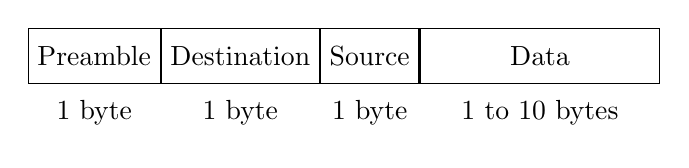
\begin{tikzpicture}
	\node [rect] (preamble) {Preamble};
	\node [rect, right=0em of preamble] (destination) {Destination};
	\node [rect, right=0em of destination] (source) {Source};
	\node [rect, right=0em of source, text width=8em] (data) {Data};
	\node [nrect, below=0em of preamble] (preamble-size) {1 byte};
	\node [nrect, below=0em of destination] (destination-size) {1 byte};
	\node [nrect, below=0em of source] (source-size) {1 byte};
	\node [nrect, below=0em of data] (data-size) {1 to 10 bytes};
\end{tikzpicture}
\\
Preamble stores information about the frame type.\\
If the preamble is set to 00000000 then it is for dhcpLite request\\
If the preamble is set to 00000001 then it is for dhcpLite granted\\
If the preamble is set to 00000010 then it is for dhcpLite rejected\\
If the preamble is set to 10000000 then it is for data transfer
\subsection{Code snippets}

\section{Test cases and Results}

\end{document}
